\section{Liczby losowe o rozkładzie równomiernym (uniform deviate)}
\begin{frame}{Liczby losowe o rozkładzie równomiernym (uniform deviate)}


	Podstawowy typ generatora liczb losowych:
	\begin{center}
	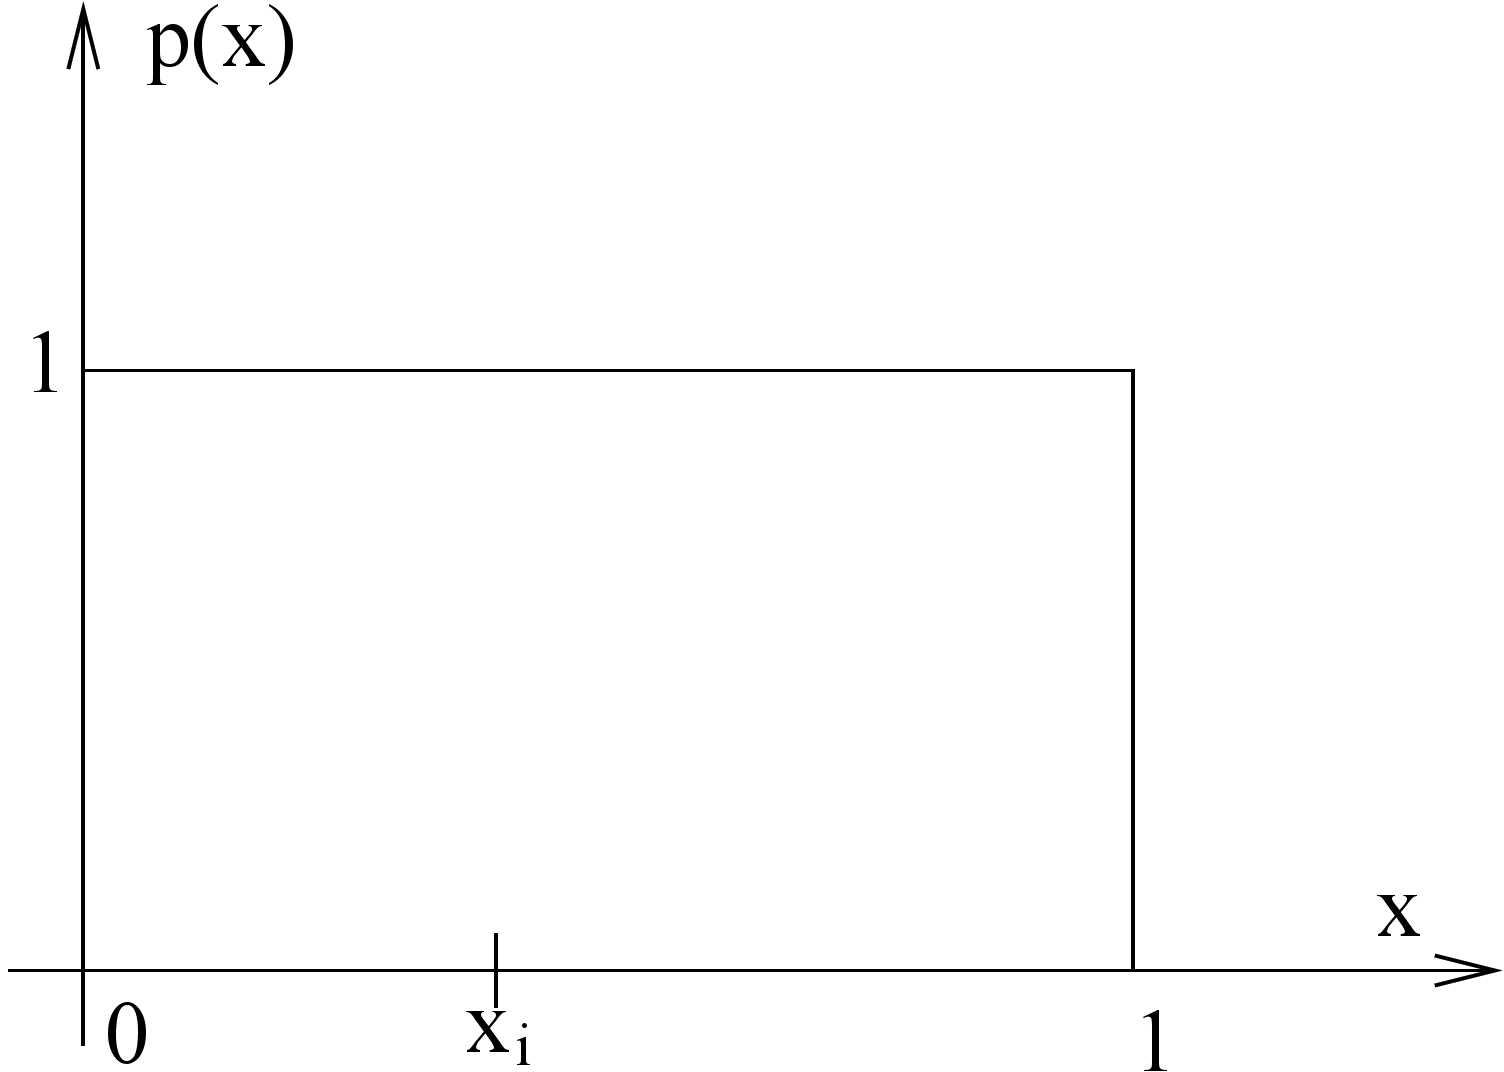
\includegraphics[scale=0.15]{img/14/14_2_img}
	\end{center}
    \end{frame}

    \begin{frame}
    \begin{exampleblock}{}
	$\{x_{i}\}-$ ciąg liczb z przedziału $(0,1)$ --równomierny na $(0,1)$, gdy:
	$$
	\forall(a,\ b)\ :\ 0\leq a\leq b\leq 1\ \lim_{N\rightarrow\infty}\frac{1}{N}\sum_{i/1}^{N}\eta_{a,b}		(x_{i})=b-a
	$$
	gdzie: $\eta_{a,b}=\left\{\begin{array}{l}
	1,\ a<x<b\\
	0,\ \mathrm{p}\mathrm{o}\mathrm{z}\mathrm{o}\mathrm{s}\mathrm{t}\mathrm{a}\mathrm{l}\mathrm{e}.
	\end{array}\right.$
	\end{exampleblock}
	W większości bibliotek programów procedura \textit{ranf}.

            \[
            	x = ranf(iseed)
            \]

	- pod $x$ podstaw następną liczbę losową \\
    - aktualizuj \textit{iseed}

	\textbf{iseed} --dowolna, zadawana przy pierwszym wywołaniu; \\
	- ta sama początkowa wartość $\Rightarrow$ ta sama sekwencja liczb pseudolosowych.
	\end{frame}
